\documentclass[letter]{article}
\usepackage[T1,T2A]{fontenc}
\usepackage[utf8]{inputenc}
\usepackage[french,english,russian]{babel}
\usepackage{graphics}
\usepackage{cmap}
\usepackage[colorlinks,linkcolor=blue]{hyperref}
\usepackage[landscape,left=0.1cm, right=0.1cm, top=0.1cm, bottom=0.1cm,paperwidth=7in,paperheight=9in]{geometry}

\usepackage[dvipsnames]{xcolor}
\usepackage{tikz}
\usepackage{calc}
\usetikzlibrary{shapes.misc}
\usepackage{varwidth}
\usepackage{fancyhdr}

\fancypagestyle{sideheading}{%
  %% Clear all headers and footers
  \fancyhf{}
  \fancyhead[LO]{%
\begin{tikzpicture}[overlay,remember picture]
      \node[fill=NavyBlue!50,text=white,
      inner ysep=8pt, inner xsep=15pt,
      rounded rectangle,
      execute at begin node={\begin{varwidth}{\textheight}},%<====
      execute at end node={\end{varwidth}},
      rotate=90]
      at ([xshift=9mm,yshift=0mm]current page.west)
      {\textsf{\textbf{WIKIMEDIA COMMONS}}};
    \end{tikzpicture}
        }
  \renewcommand{\headrulewidth}{0pt}
  \renewcommand{\footrulewidth}{0pt}
  \fancyfoot[R]{}
}

\pagestyle{sideheading}
\newcommand{\myhref}[2]{\selectlanguage{french}\textcolor{blue}{\href{#1}{\selectlanguage{russian}\textcolor{blue}{#2}}}\selectlanguage{russian}}
\newcommand{\pictitle}[4]{\myhref{#4}{\textsf{\textbf{#1.}}} \textit{#2.} #3.\bigskip}
\newenvironment{myframe}{\begin{center}}{\end{center}\newpage}

\author{Vitaly Repin \thanks{Thanks to Prof. Michael S. Roth, Wesleyan University and Coursera}}
\title{The Modern and the Postmodern\\  \textit{\small Visual arts discussed in the course on the Modern and the Postmodern @ Wesleyan University}}
\date{September 2013}

\begin{document}
\maketitle
\newpage

\begin{myframe}
\pictitle{La Mort de Sardanapale (Death of Sardanapalus, Смерть Сарданапала)}{Eugène Delacroix, 1827}{Louvre, Paris}{http://commons.wikimedia.org/wiki/File:Delacroix_-_La_Mort_de_Sardanapale_(1827).jpg}

\resizebox{.86\textwidth}{!}{\includegraphics{Delacroix_-_La_Mort_de_Sardanapale_(1827)}}
\end{myframe}

\begin{myframe}
\pictitle{Scène des massacres de Scio (The Massacre at Chios, Резня на Хиосе)}{Eugène Delacroix, 1824}{Louvre, Paris}{http://commons.wikimedia.org/wiki/File:Eugène_Delacroix_-_Le_Massacre_de_Scio.jpg}

\resizebox{!}{.95\textheight}{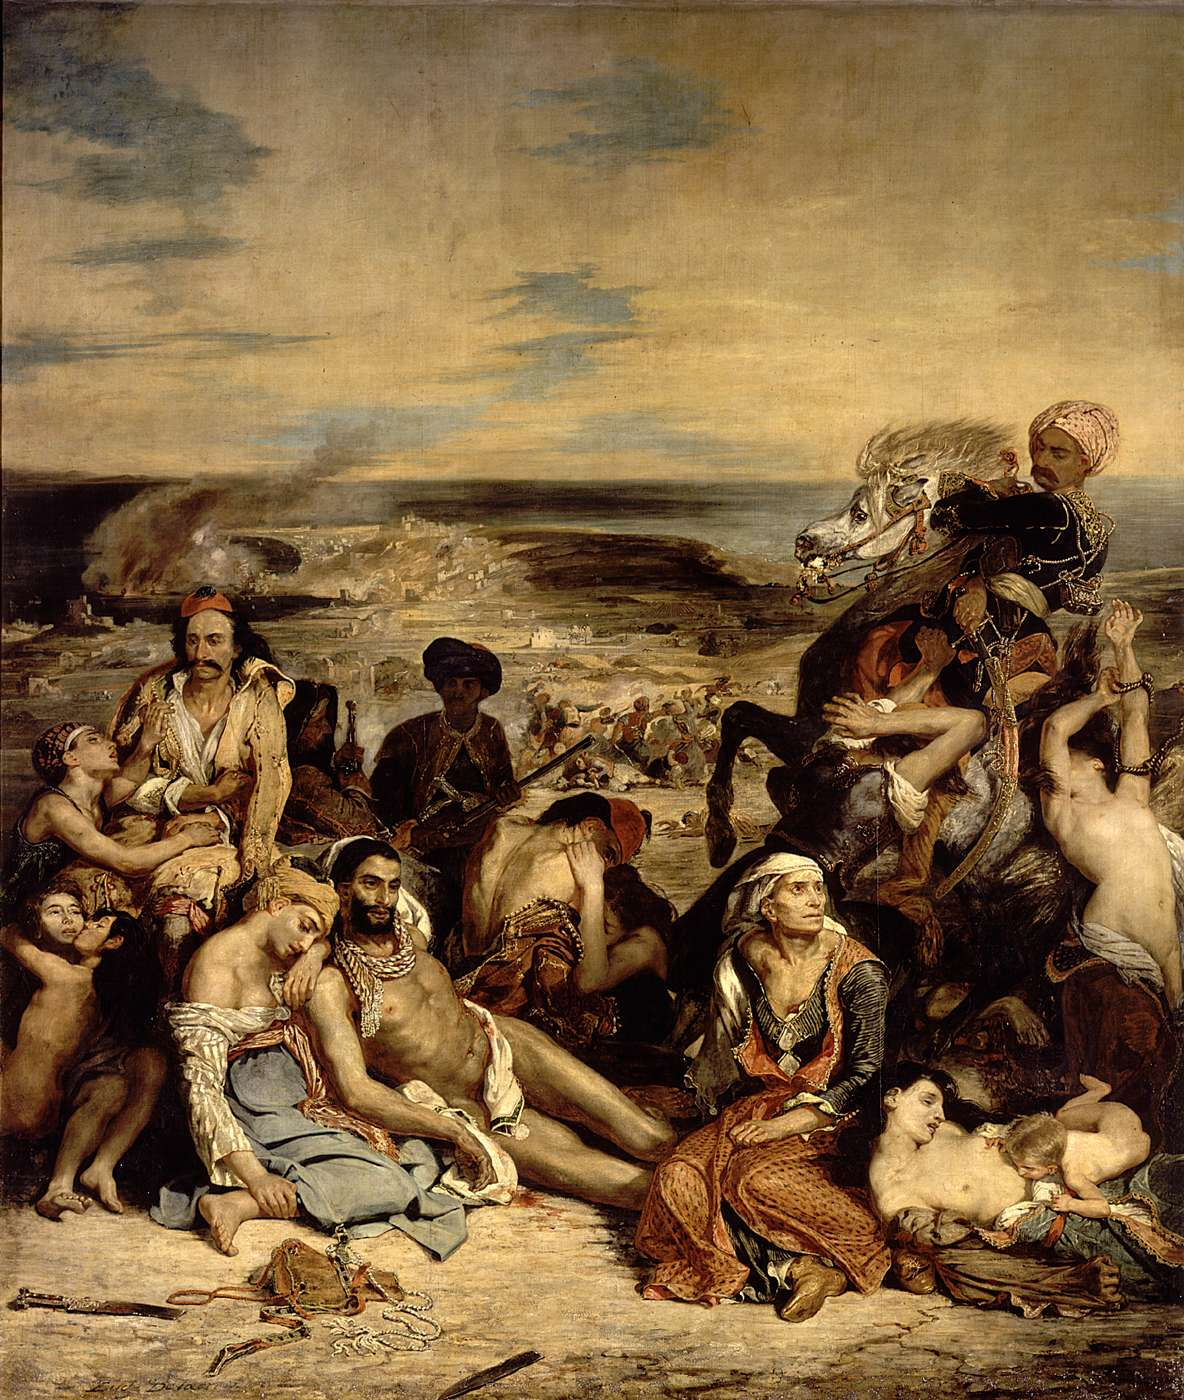
\includegraphics{Eugene_Delacroix_-_Le_Massacre_de_Scio}}
\end{myframe}

\begin{myframe}
\pictitle{La Liberté guidant le peuple (Liberty Leading the People; Свобода, ведущая народ; Свобода на баррикадах)}{\\ Eugène Delacroix, 1830}{Louvre-Lens, Lens}{http://commons.wikimedia.org/wiki/File:Eugène_Delacroix_-_Le_28_Juillet._La_Liberté_guidant_le_peuple.jpg}

\resizebox{0.87\textwidth}{!}{\includegraphics{Eugene_Delacroix_-_Le_28_Juillet_La_Liberte_guidant_le_peuple.jpg}}
\end{myframe}

\begin{myframe}
\pictitle{Le Désespéré (Self portrait, Автопортрет)}{Gustave Courbet, 1841}{Private collection}{http://commons.wikimedia.org/wiki/File:Gustave_Courbet_-_Le_Désespéré_(1843).jpg}

\resizebox{!}{.92\textheight}{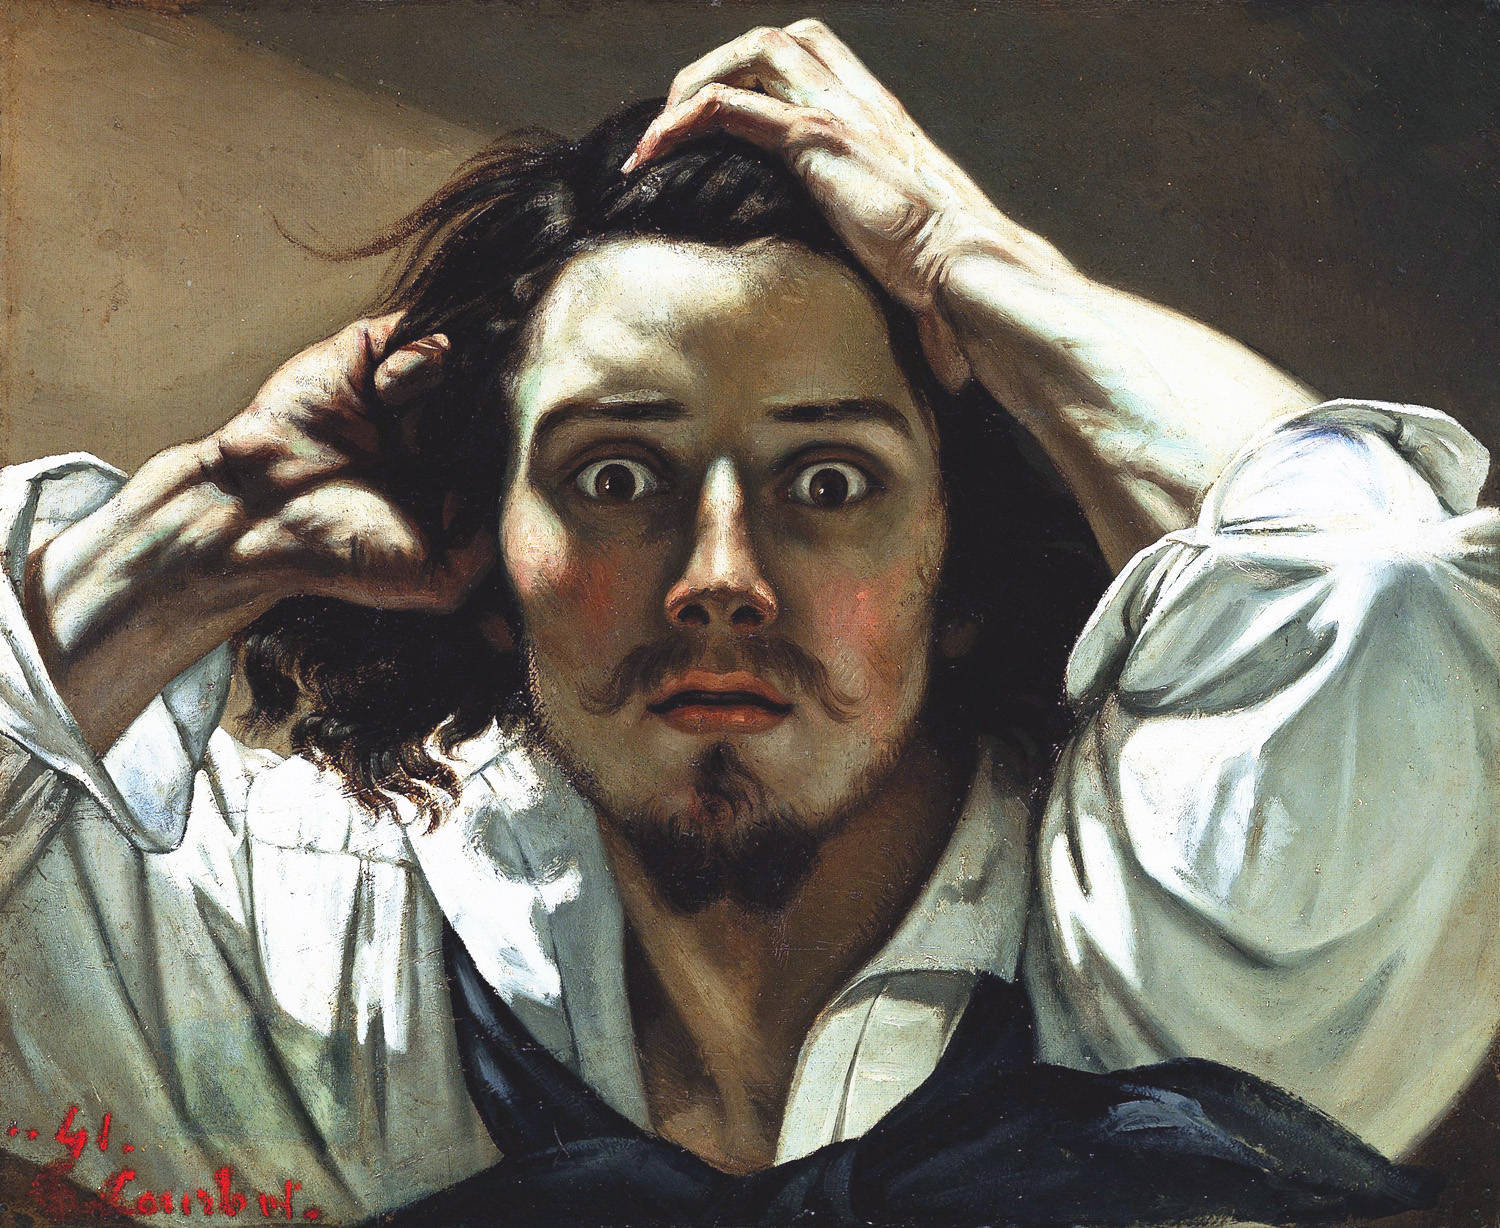
\includegraphics{Gustave_Courbet_-_self_(1843)}}
\end{myframe}

\begin{myframe}
\pictitle{Steinhauer (Stone Breaker, Камнетёс)}{Gustave Courbet, 1849}{Private collection, Milan}{http://commons.wikimedia.org/wiki/File:Gustave_Courbet_040.jpg}

\resizebox{!}{.92\textheight}{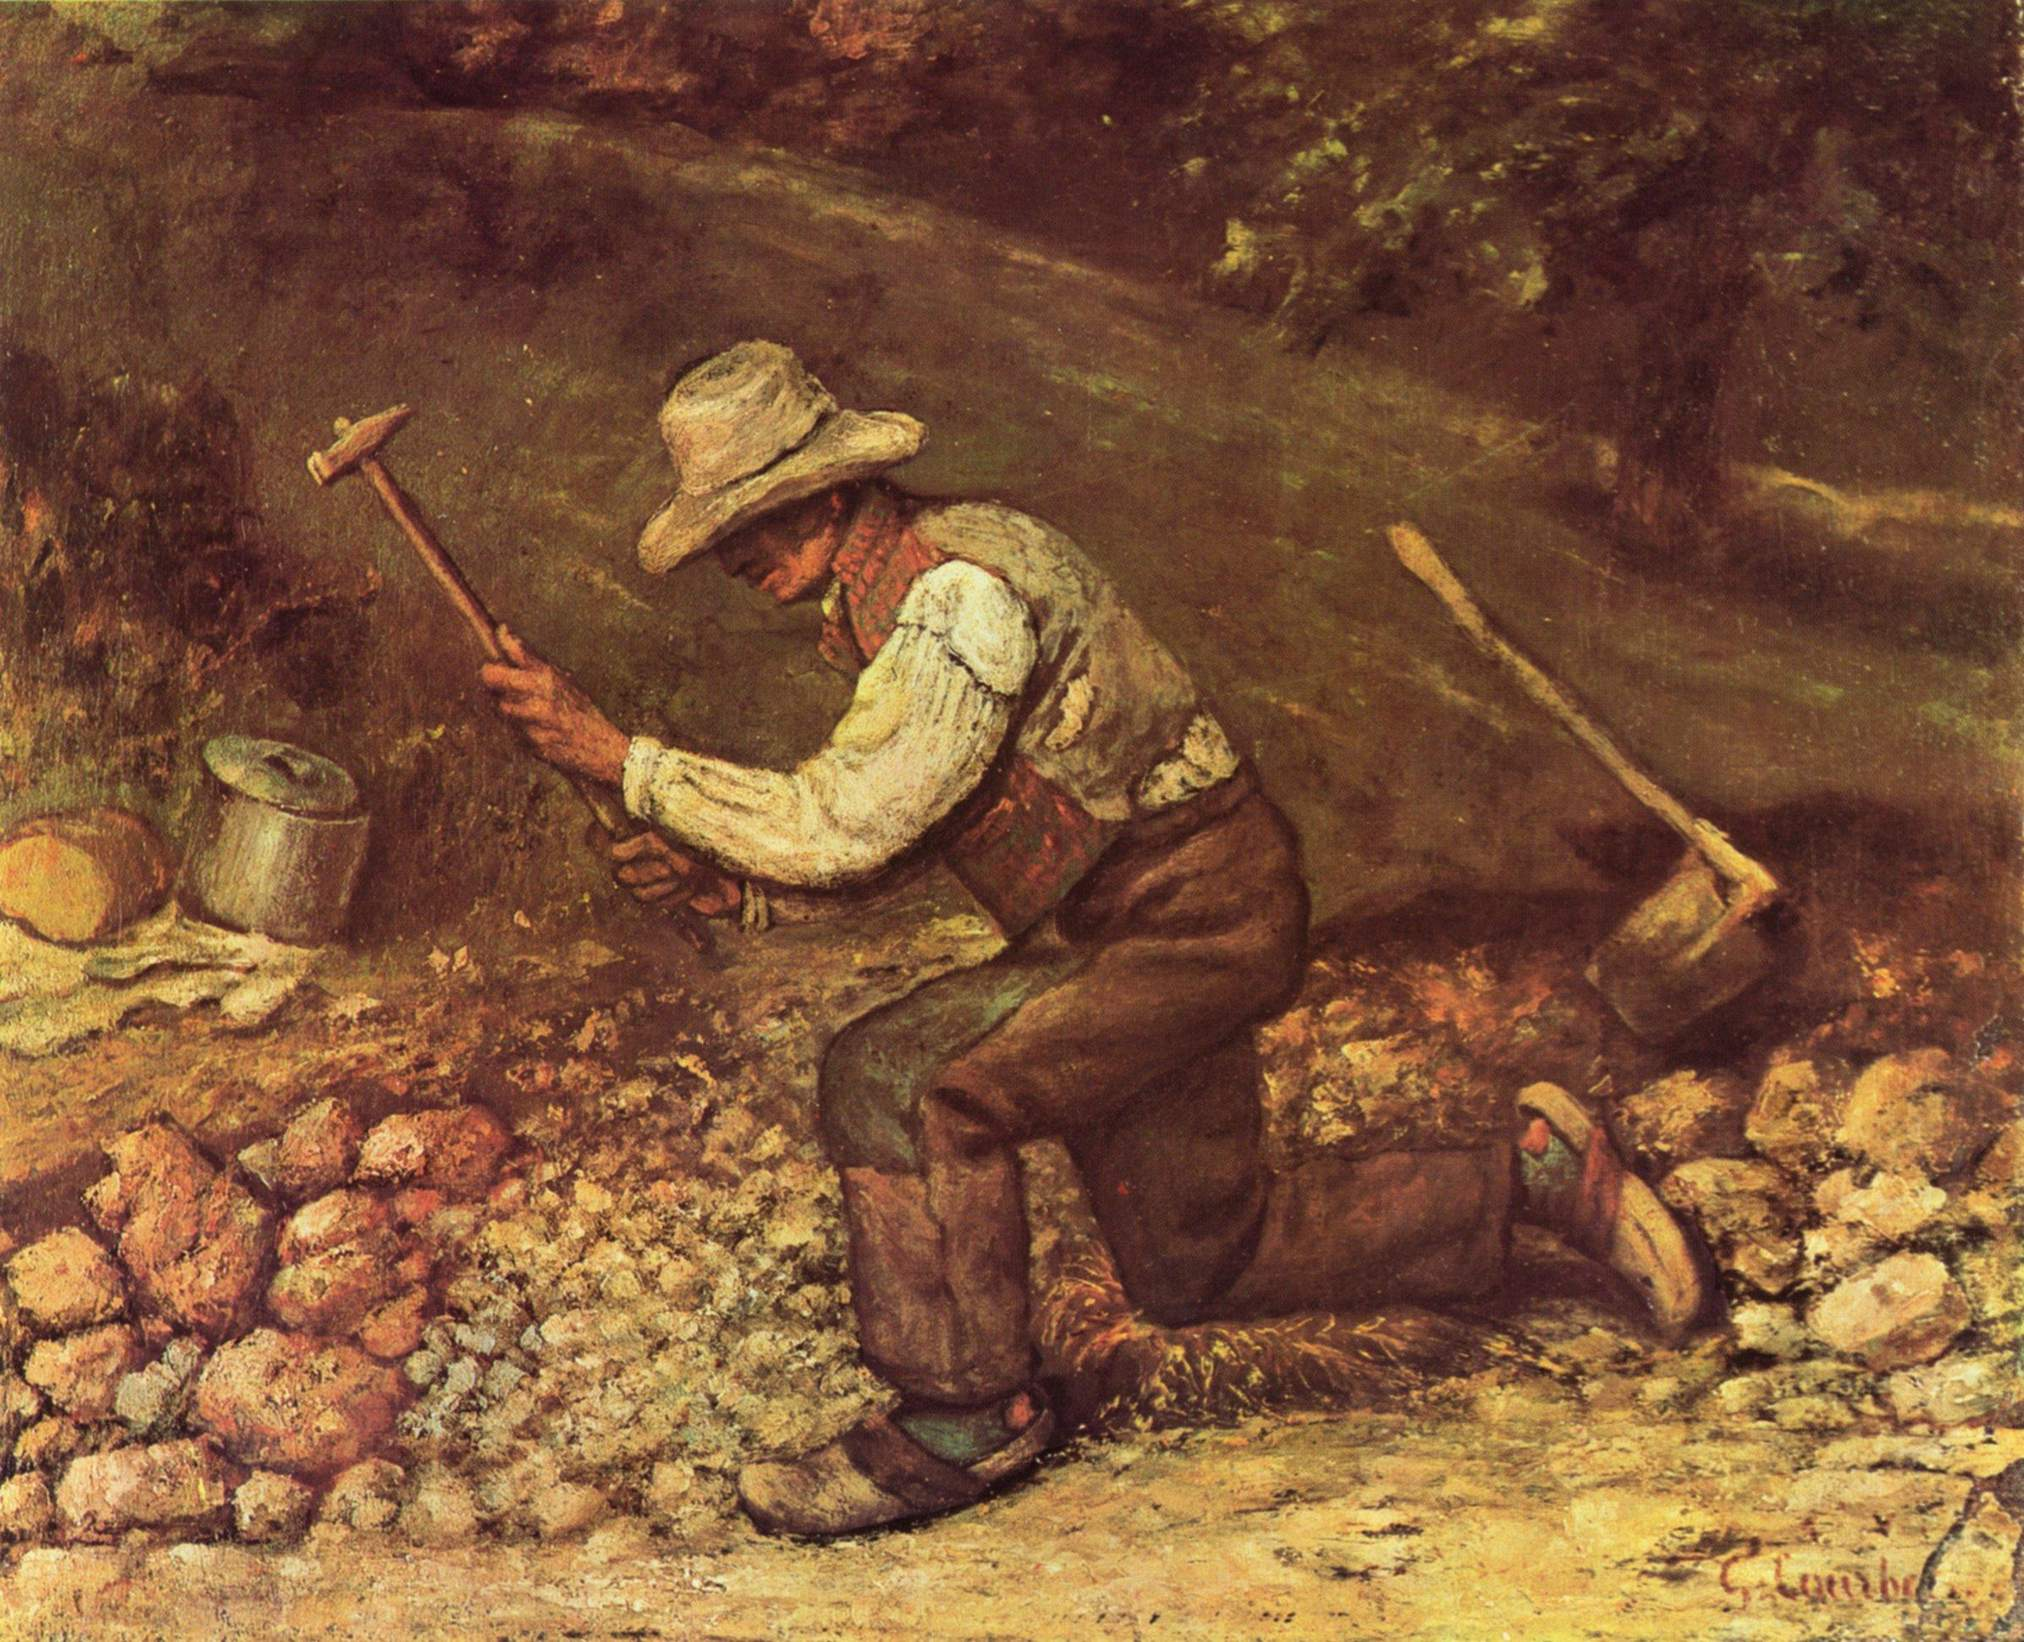
\includegraphics{Gustave_Courbet_040.jpg}}
\end{myframe}

\begin{myframe}
\pictitle{Le Sommeil (The Sleepers, Спящие)}{Gustave Courbet, 1866}{Petit Palais, Paris}{http://commons.wikimedia.org/wiki/File:Courbet_Sleep.jpg}

\resizebox{!}{.76\textheight}{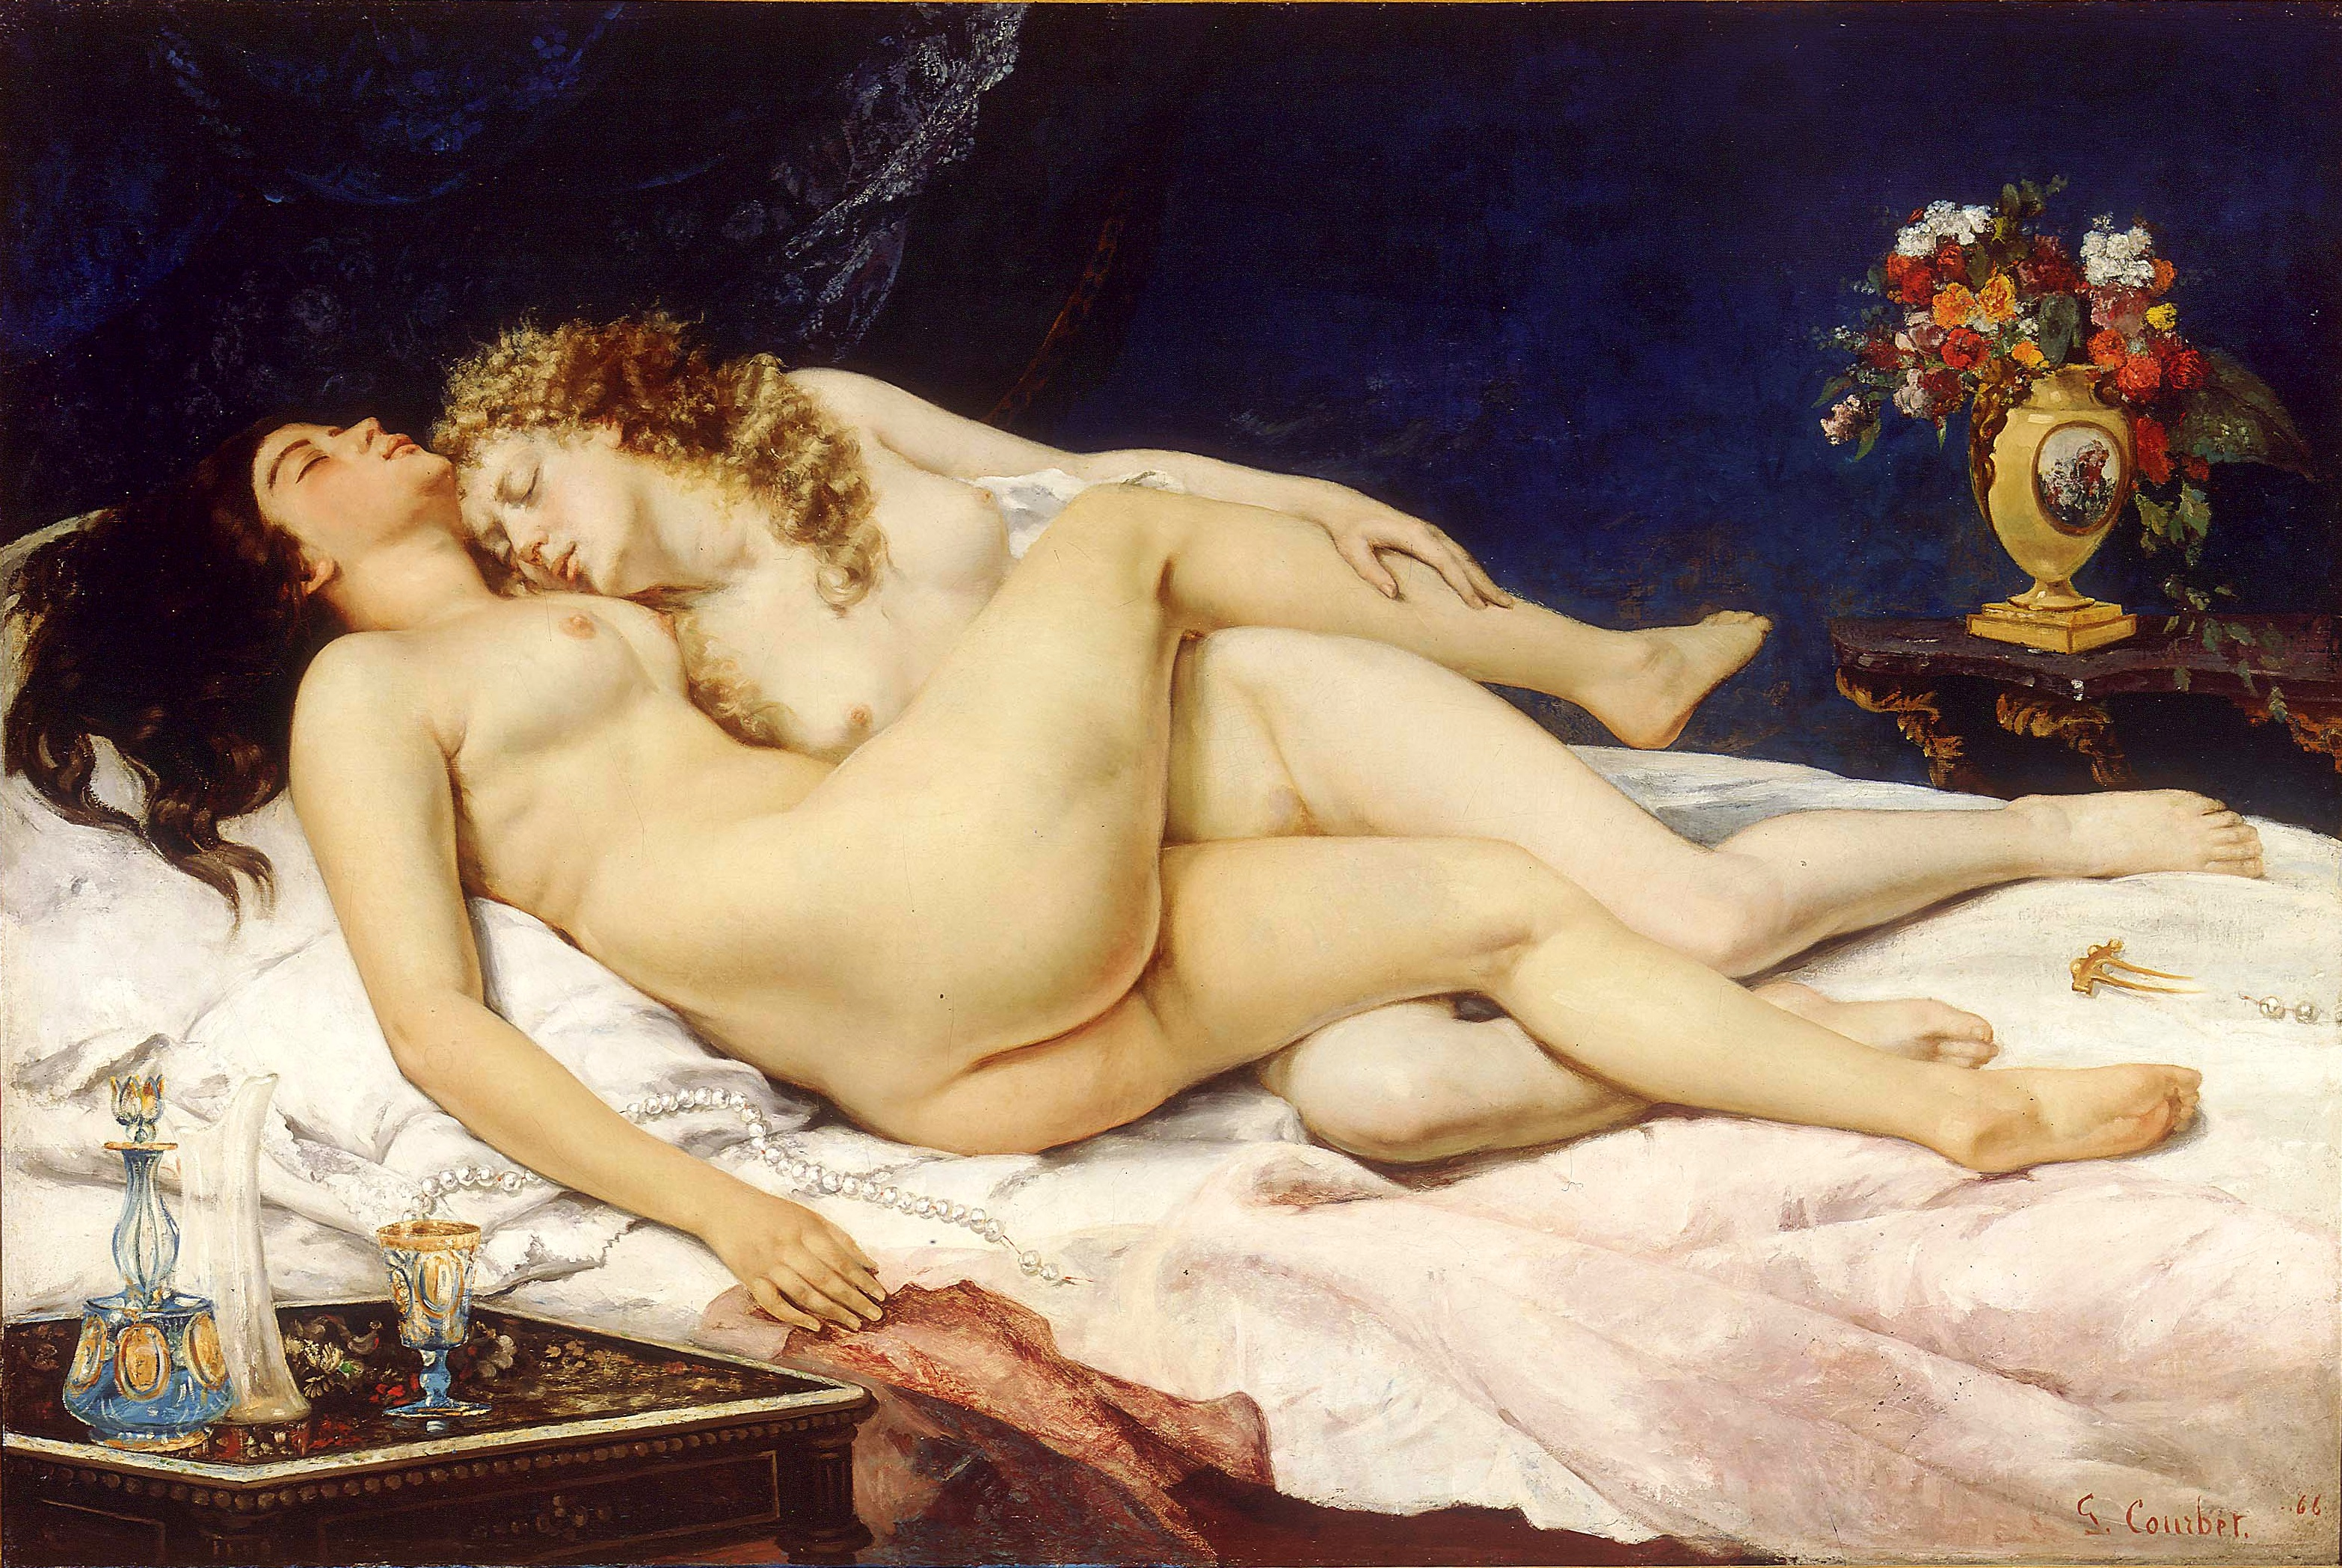
\includegraphics{Courbet_Sleep.jpg}}
\end{myframe}


\begin{myframe}
\pictitle{Un enterrement à Ornans (A Burial At Ornans, Похороны в Орнане)}{Gustave Courbet, 1850}{Musée d'Orsay, Paris}{http://commons.wikimedia.org/wiki/File:Gustave_Courbet_-_A_Burial_at_Ornans_-_Google_Art_Project_2.jpg}

\resizebox{.87\textwidth}{!}{\includegraphics{Gustave_Courbet_-_A_Burial_at_Ornans_-_Google_Art_Project_2.jpg}}
\end{myframe}

\begin{myframe}
\pictitle{Segelboote in Argenteuil (Boating in Argenteuil, Яхты в Аржантёйе)}{Édouard Manet, 1874}{National Museum Cardiff, Wales}{http://commons.wikimedia.org/wiki/File:Édouard_Manet_-_Segelboote_in_Argenteuil.jpg}

\resizebox{0.87\textwidth}{!}{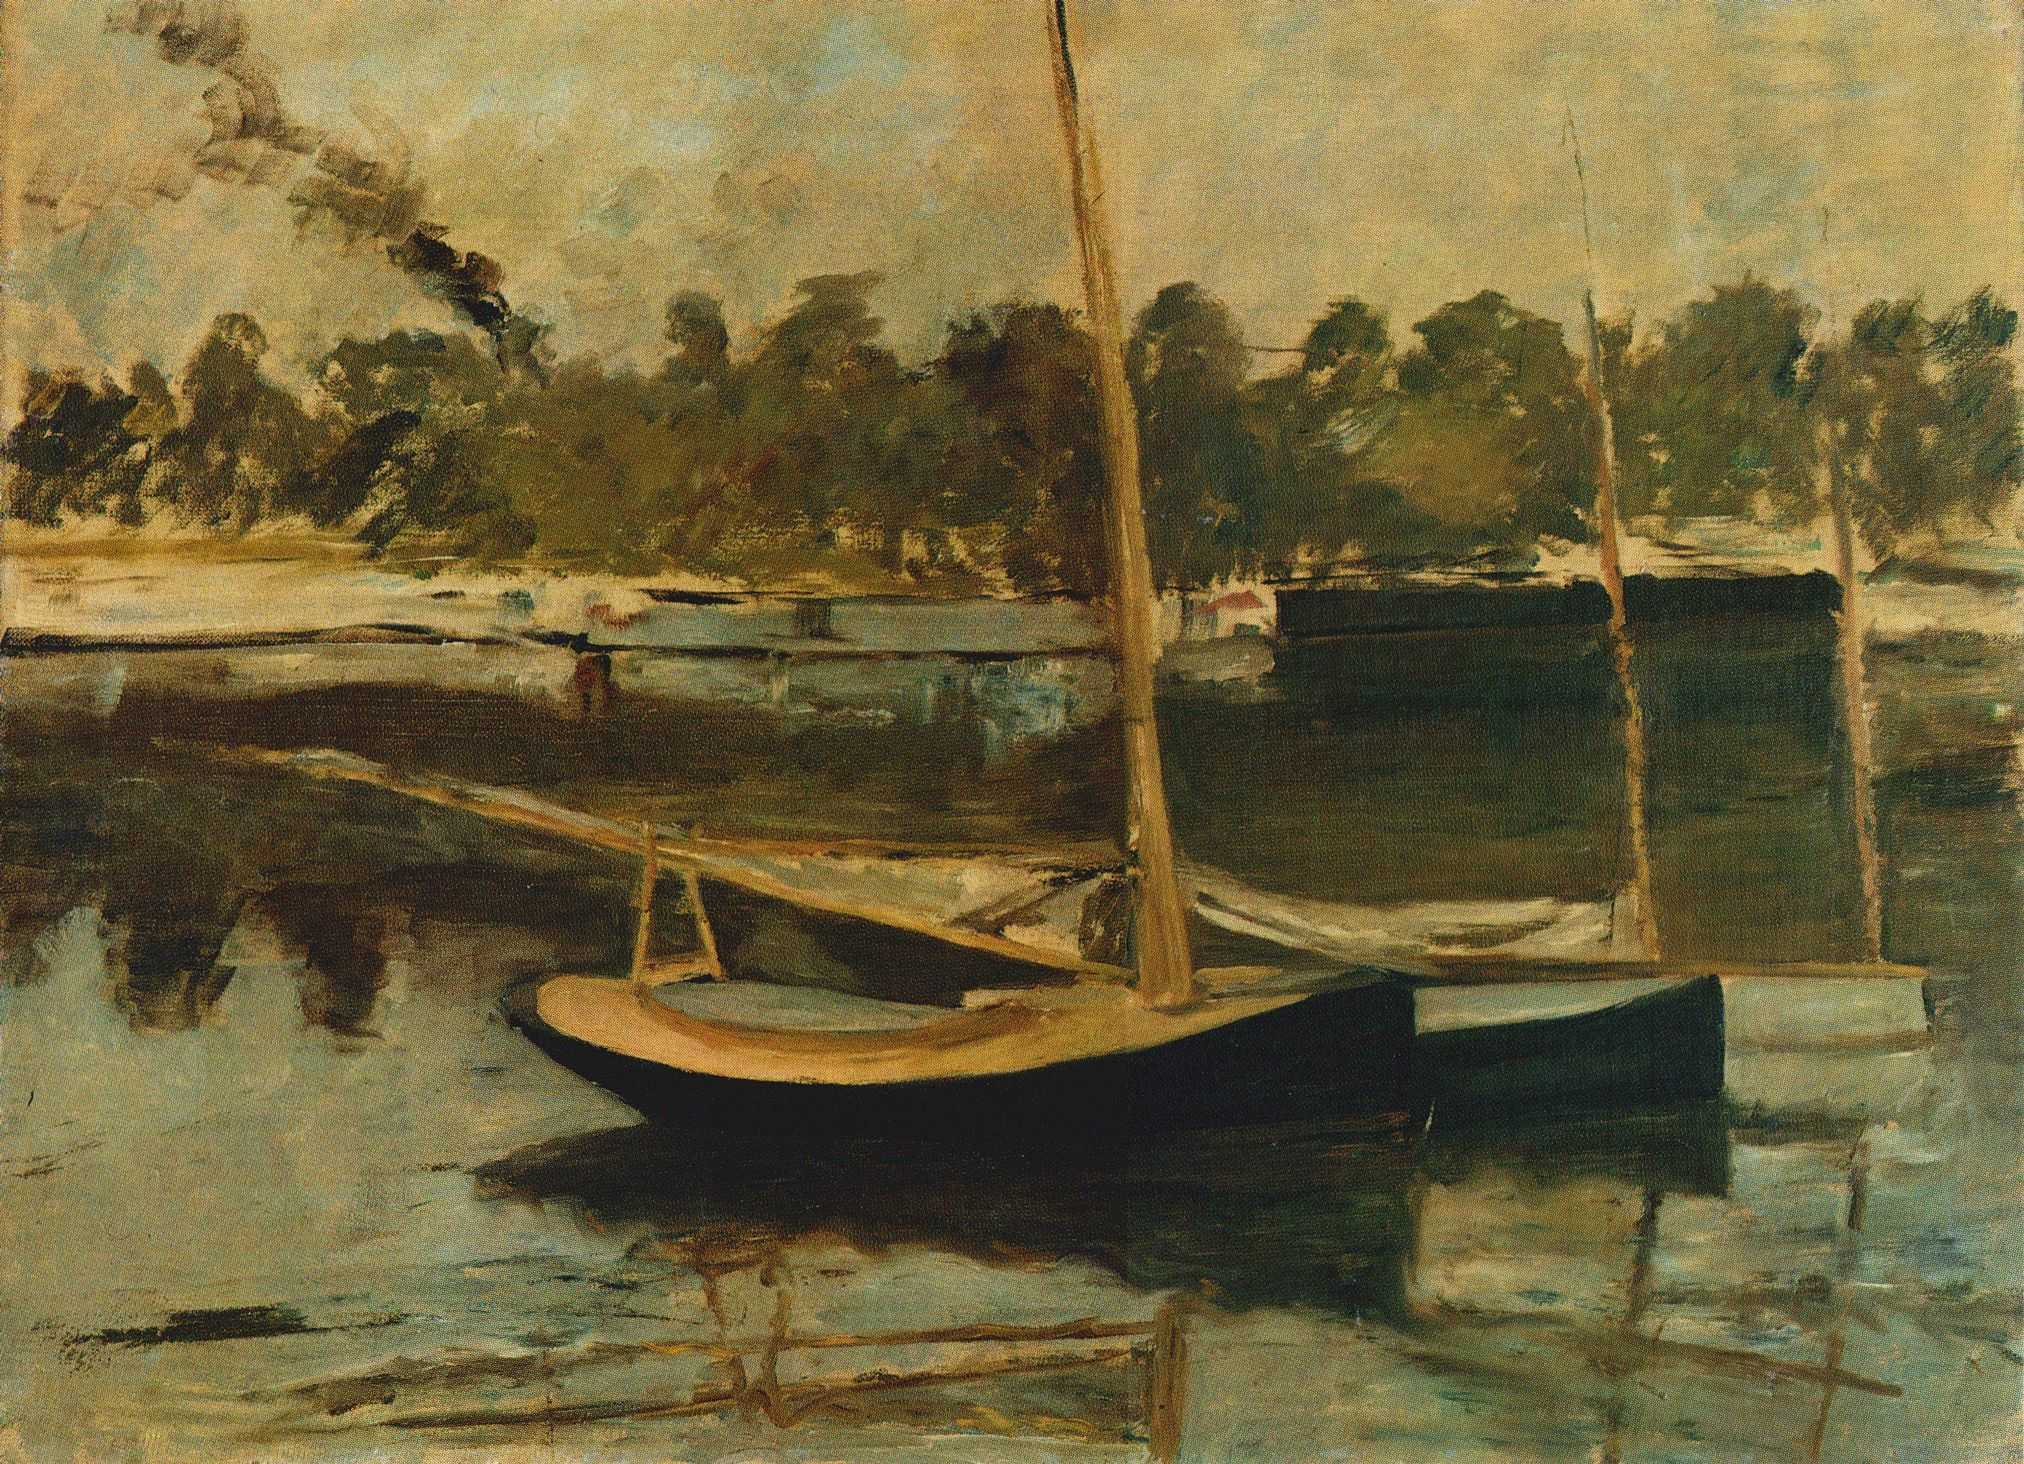
\includegraphics{Edouard_Manet_-_Segelboote_in_Argenteuil.jpg}}
\end{myframe}

\begin{myframe}
\pictitle{La Musique aux Tuileries  (Music in the Tuileries, Музыка в саду Тюильри)}{Édouard Manet, 1862}{The Hugh Lane, Dublin}{http://en.wikipedia.org/wiki/File:MANET_-_Música_en_las_Tullerías_(National_Gallery,_Londres,_1862).jpg}

\resizebox{!}{0.72\textheight}{\includegraphics{MANET_-_Musica_en_las_Tullerias_(National_Gallery,_Londres,_1862).jpg}}
\end{myframe}

\begin{myframe}
\pictitle{Le Chemin de fer (The Railway, Железная дорога)}{Édouard Manet, 1873}{National Gallery of Art, Washington}{http://en.wikipedia.org/wiki/File:Edouard_Manet_-_Le_Chemin_de_fer_-_Google_Art_Project.jpg}

\resizebox{!}{.92\textheight}{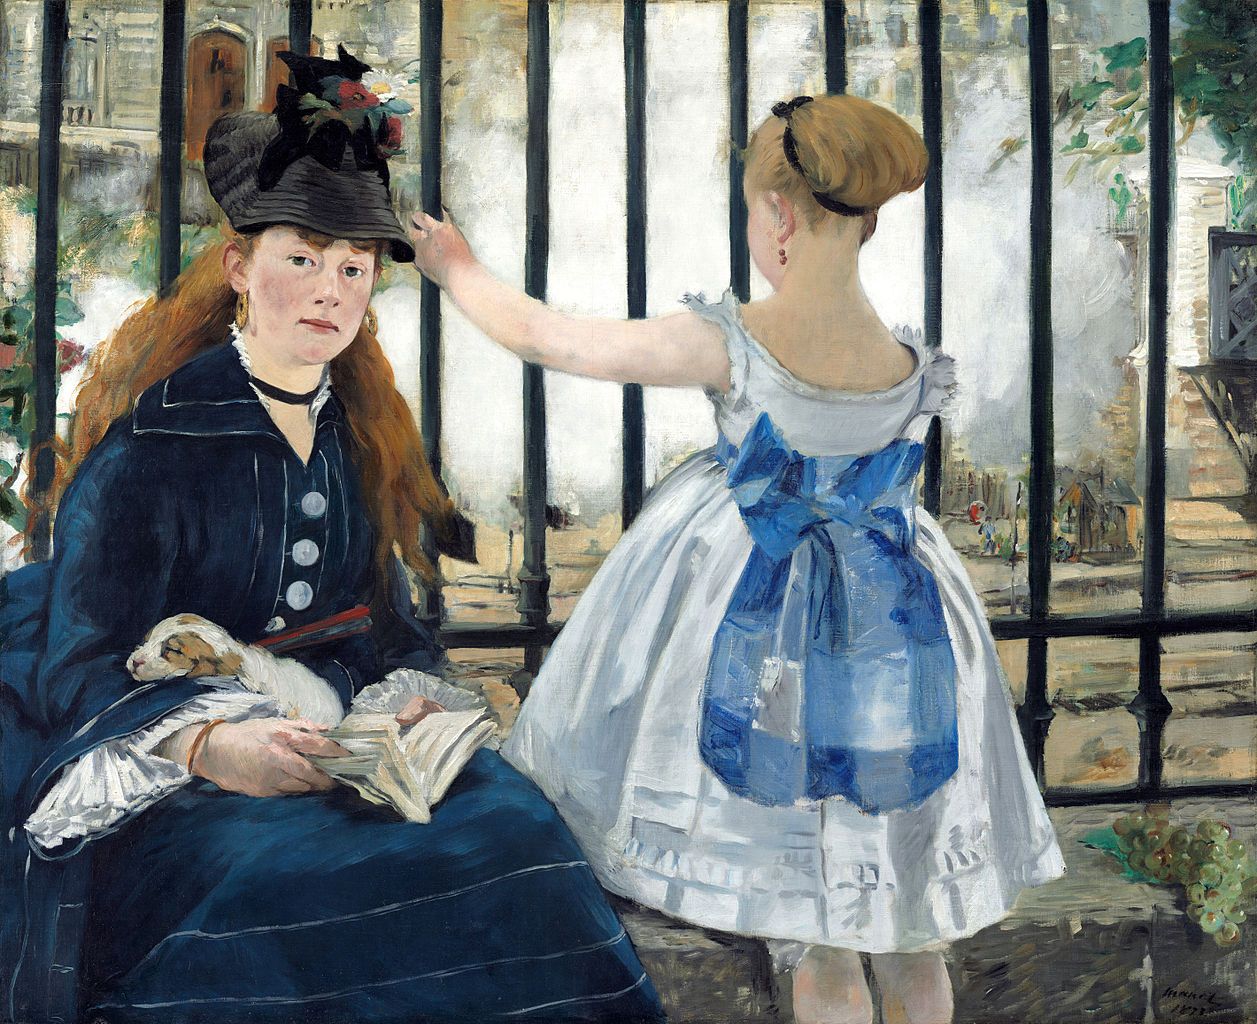
\includegraphics{Edouard_Manet_-_Le_Chemin_de_fer_-_Google_Art_Project.jpg}}
\end{myframe}

\begin{myframe}
\pictitle{Le déjeuner sur l'herbe (The Luncheon on the Grass, Завтрак на траве)}{Édouard Manet, 1863}{Musée d'Orsay, Paris}{http://en.wikipedia.org/wiki/File:Édouard_Manet_-_Le_Déjeuner_sur_l'herbe.jpg}

\resizebox{!}{.89\textheight}{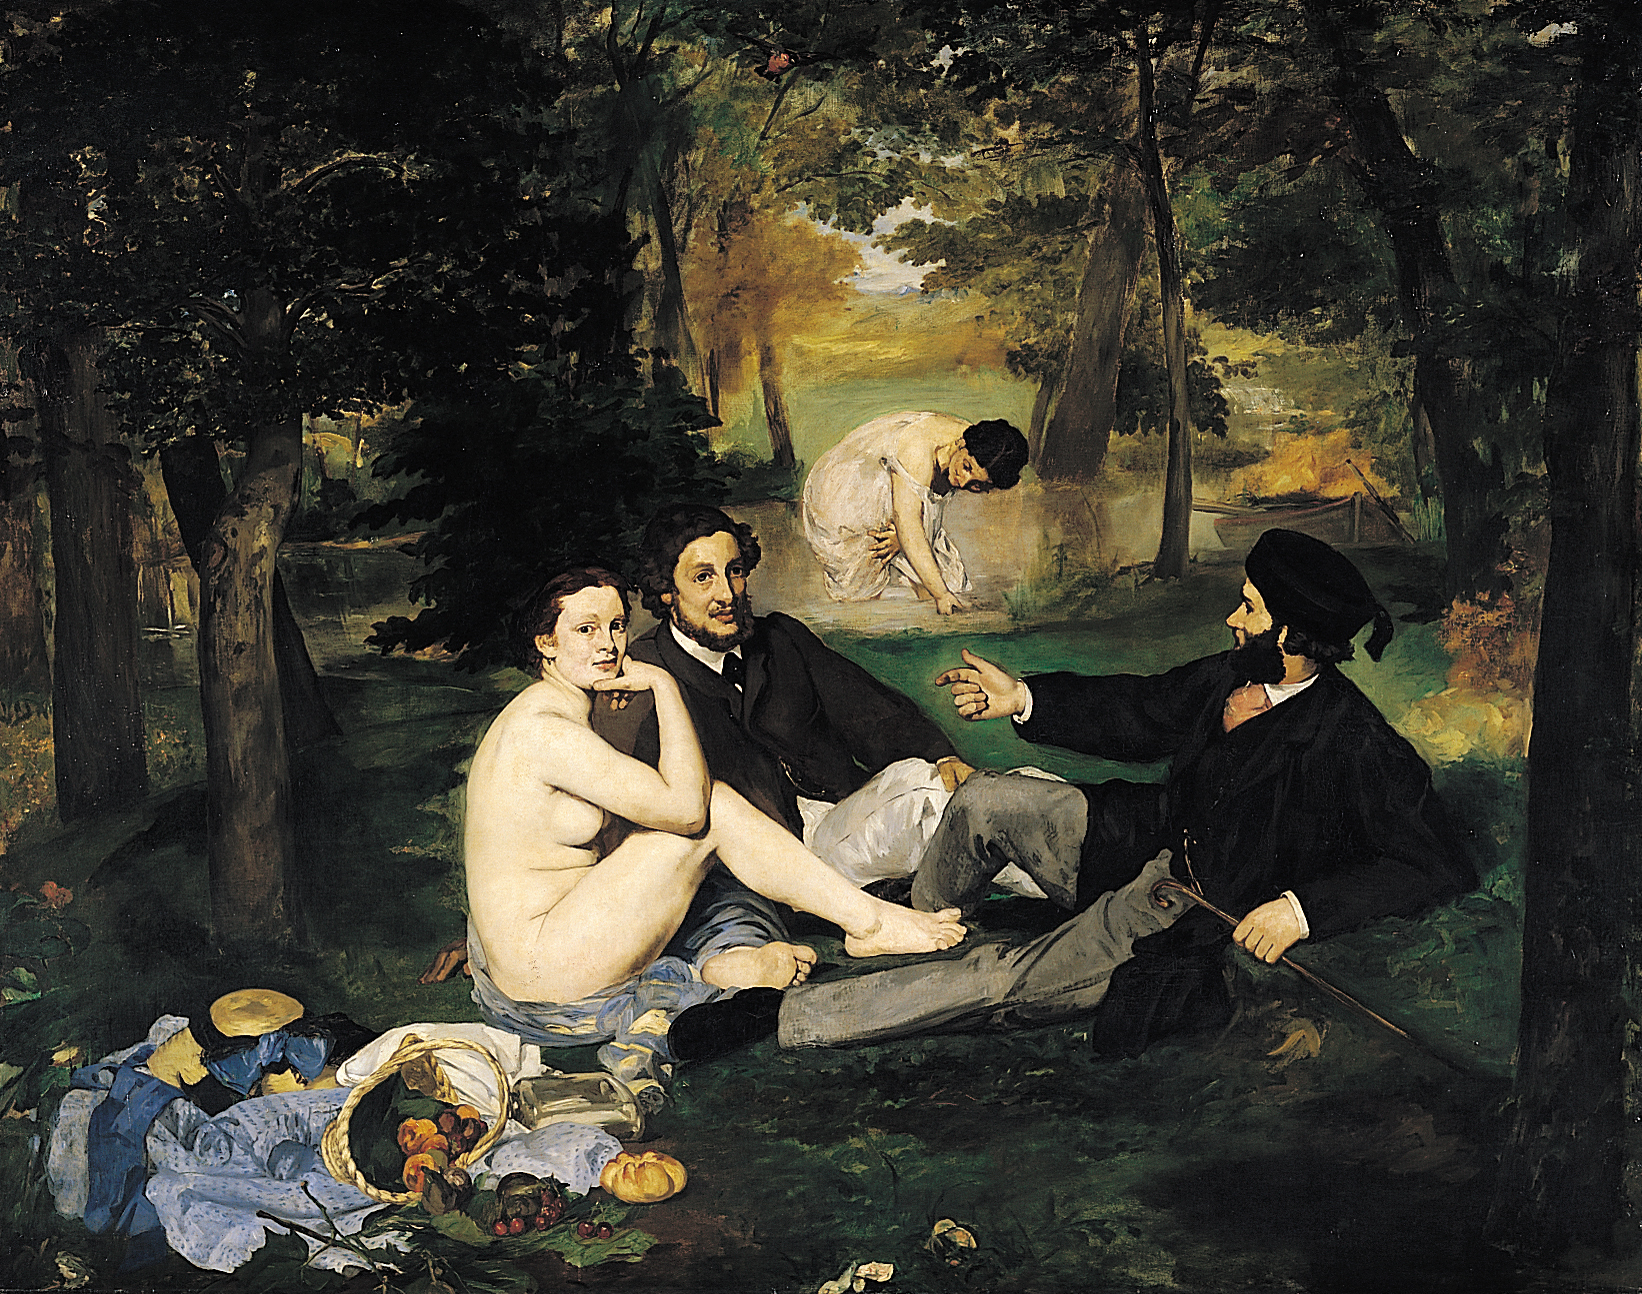
\includegraphics{Edouard_Manet_-_Le_Dejeuner_sur_lherbe.jpg}}
\end{myframe}

\begin{myframe}
\pictitle{Olympia (Olympia, Олимпия)}{Édouard Manet, 1863}{Musée d'Orsay, Paris}{http://en.wikipedia.org/wiki/File:Edouard_Manet_-_Olympia_-_Google_Art_Project_3.jpg}

\resizebox{.87\textwidth}{!}{\includegraphics{Edouard_Manet_-_Olympia_-_Google_Art_Project_3.jpg}}
\end{myframe}

\begin{myframe}
\pictitle{Portait de Baudelaire (Portrait of Charles Baudelaire, Портрет Шарля Бодлера)}{\\ Gustave Courbet, 1849}{Musée Fabre, Montpellier}{http://en.wikipedia.org/wiki/File:Gustave_Courbet_033.jpg}

\resizebox{!}{.92\textheight}{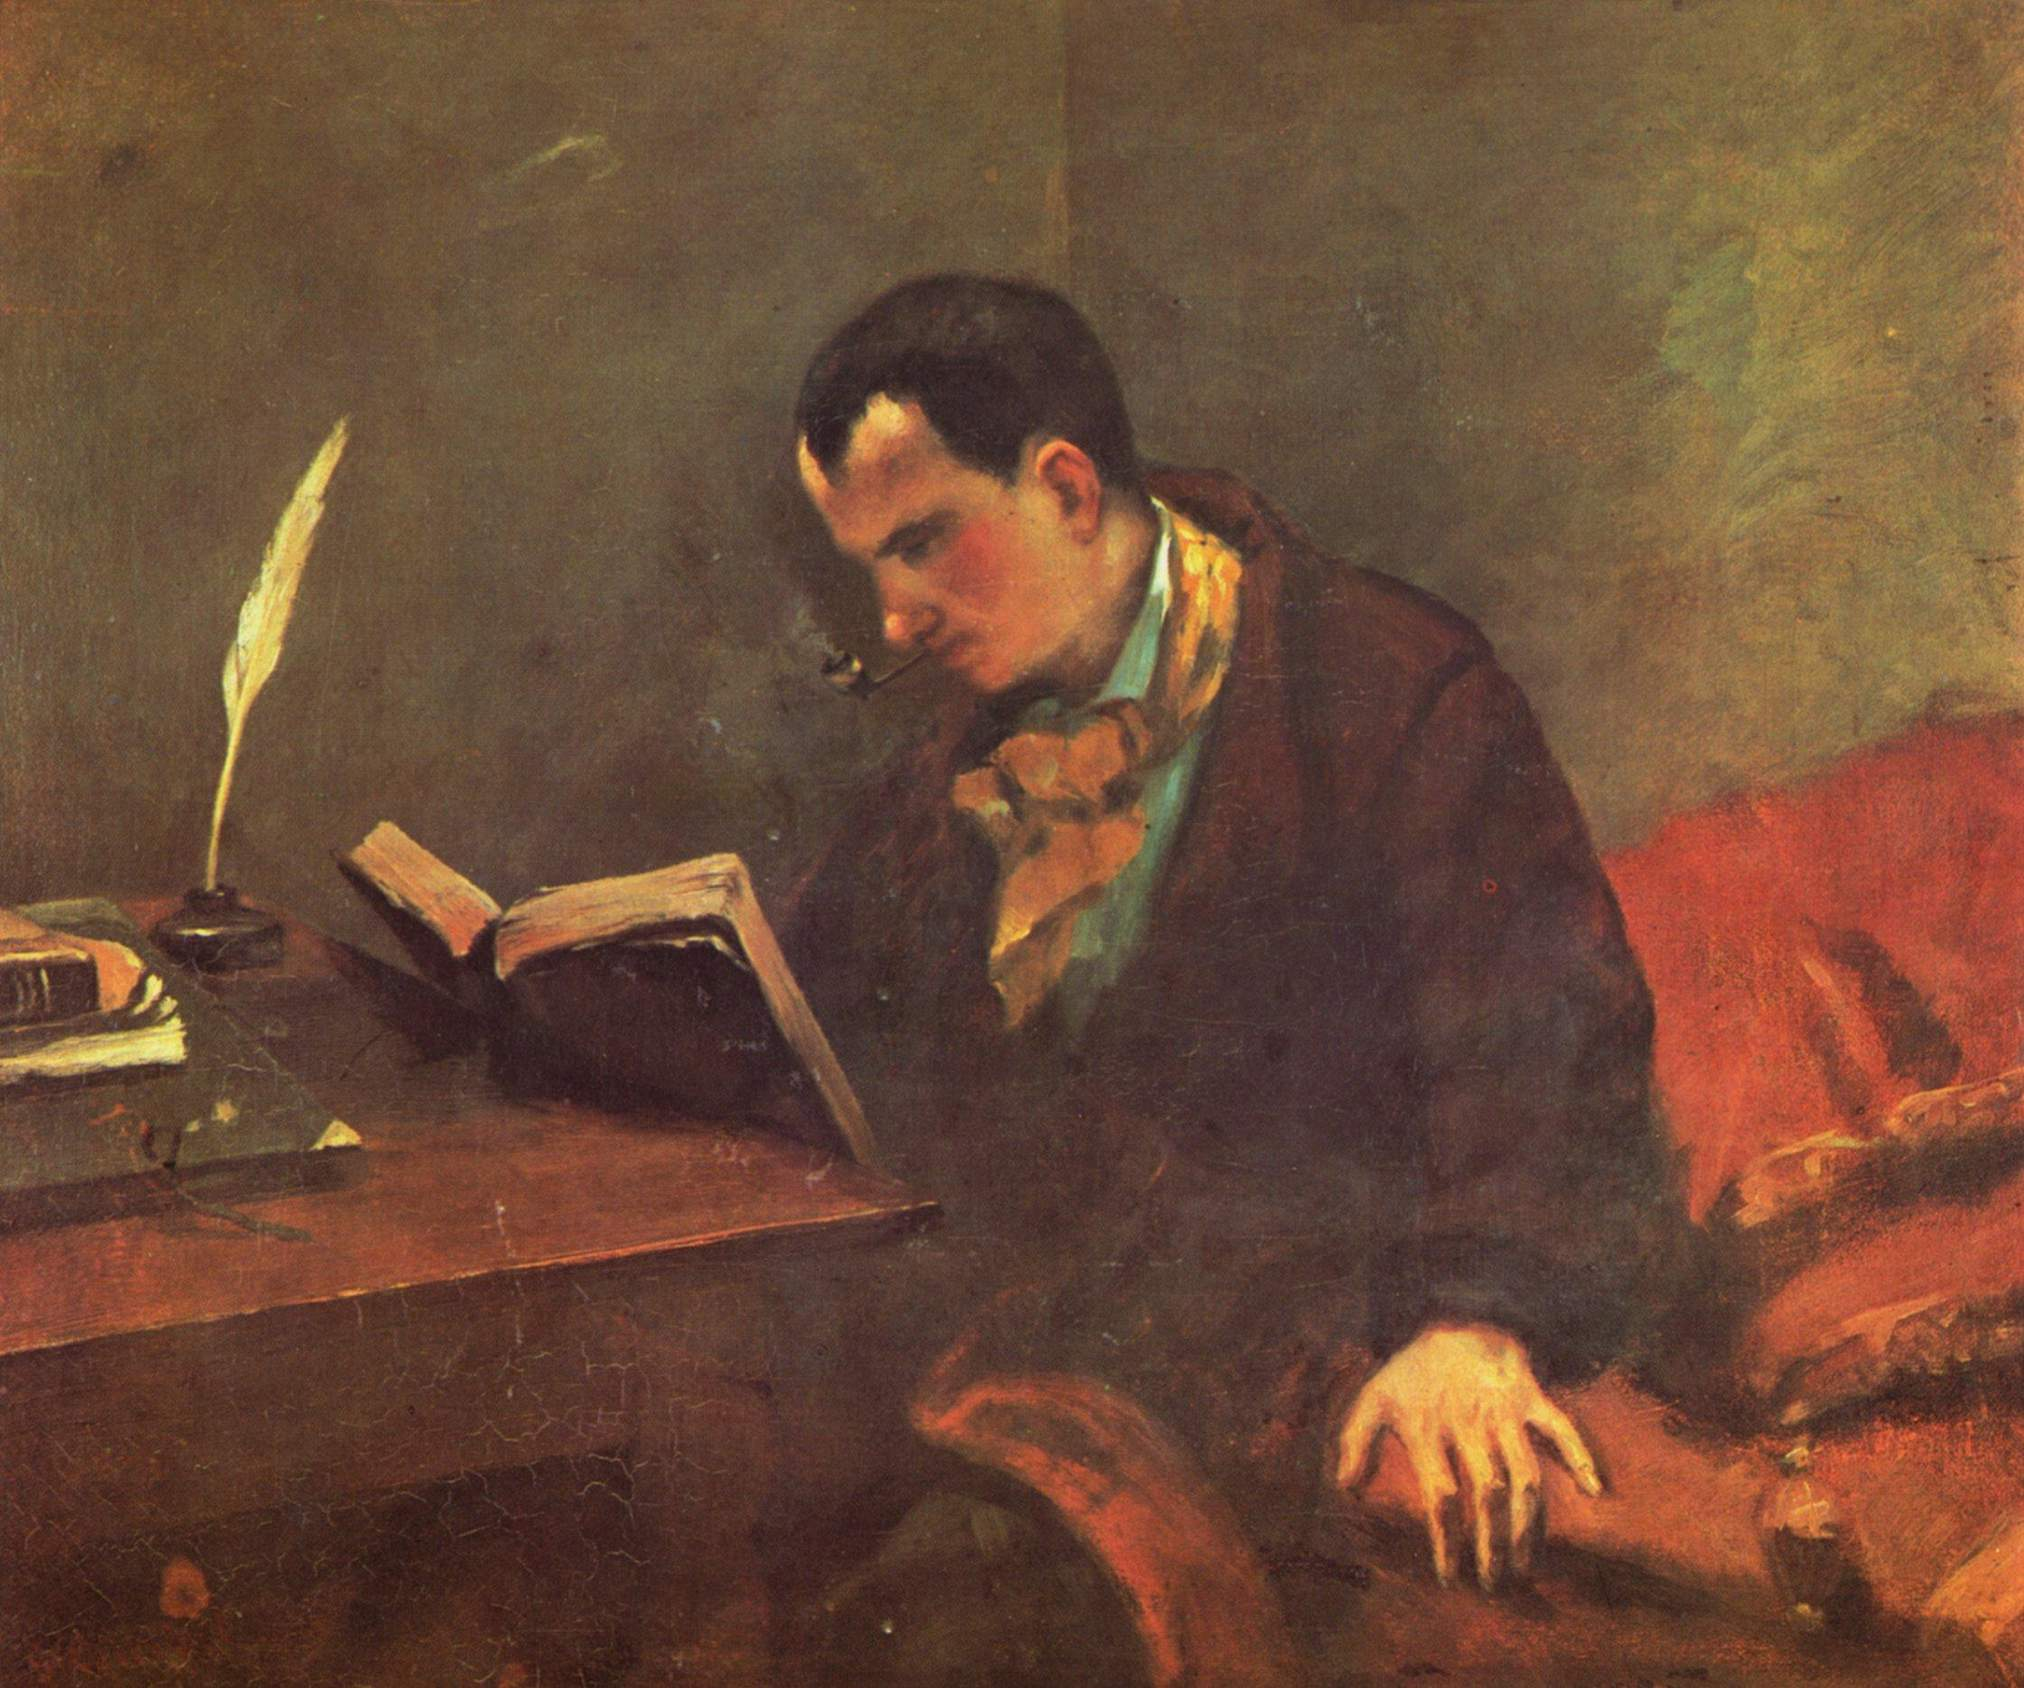
\includegraphics{Gustave_Courbet_033.jpg}}
\end{myframe}

\begin{myframe}
\pictitle{La Loge de l'opéra (Ложа)}{Constantin Guys}{Albertina, Vienna}{http://commons.wikimedia.org/wiki/File:Constantin-Ernest-Adolphe-Hyacinthe_Guys_001.jpg?uselang=ru}

\resizebox{.88\textwidth}{!}{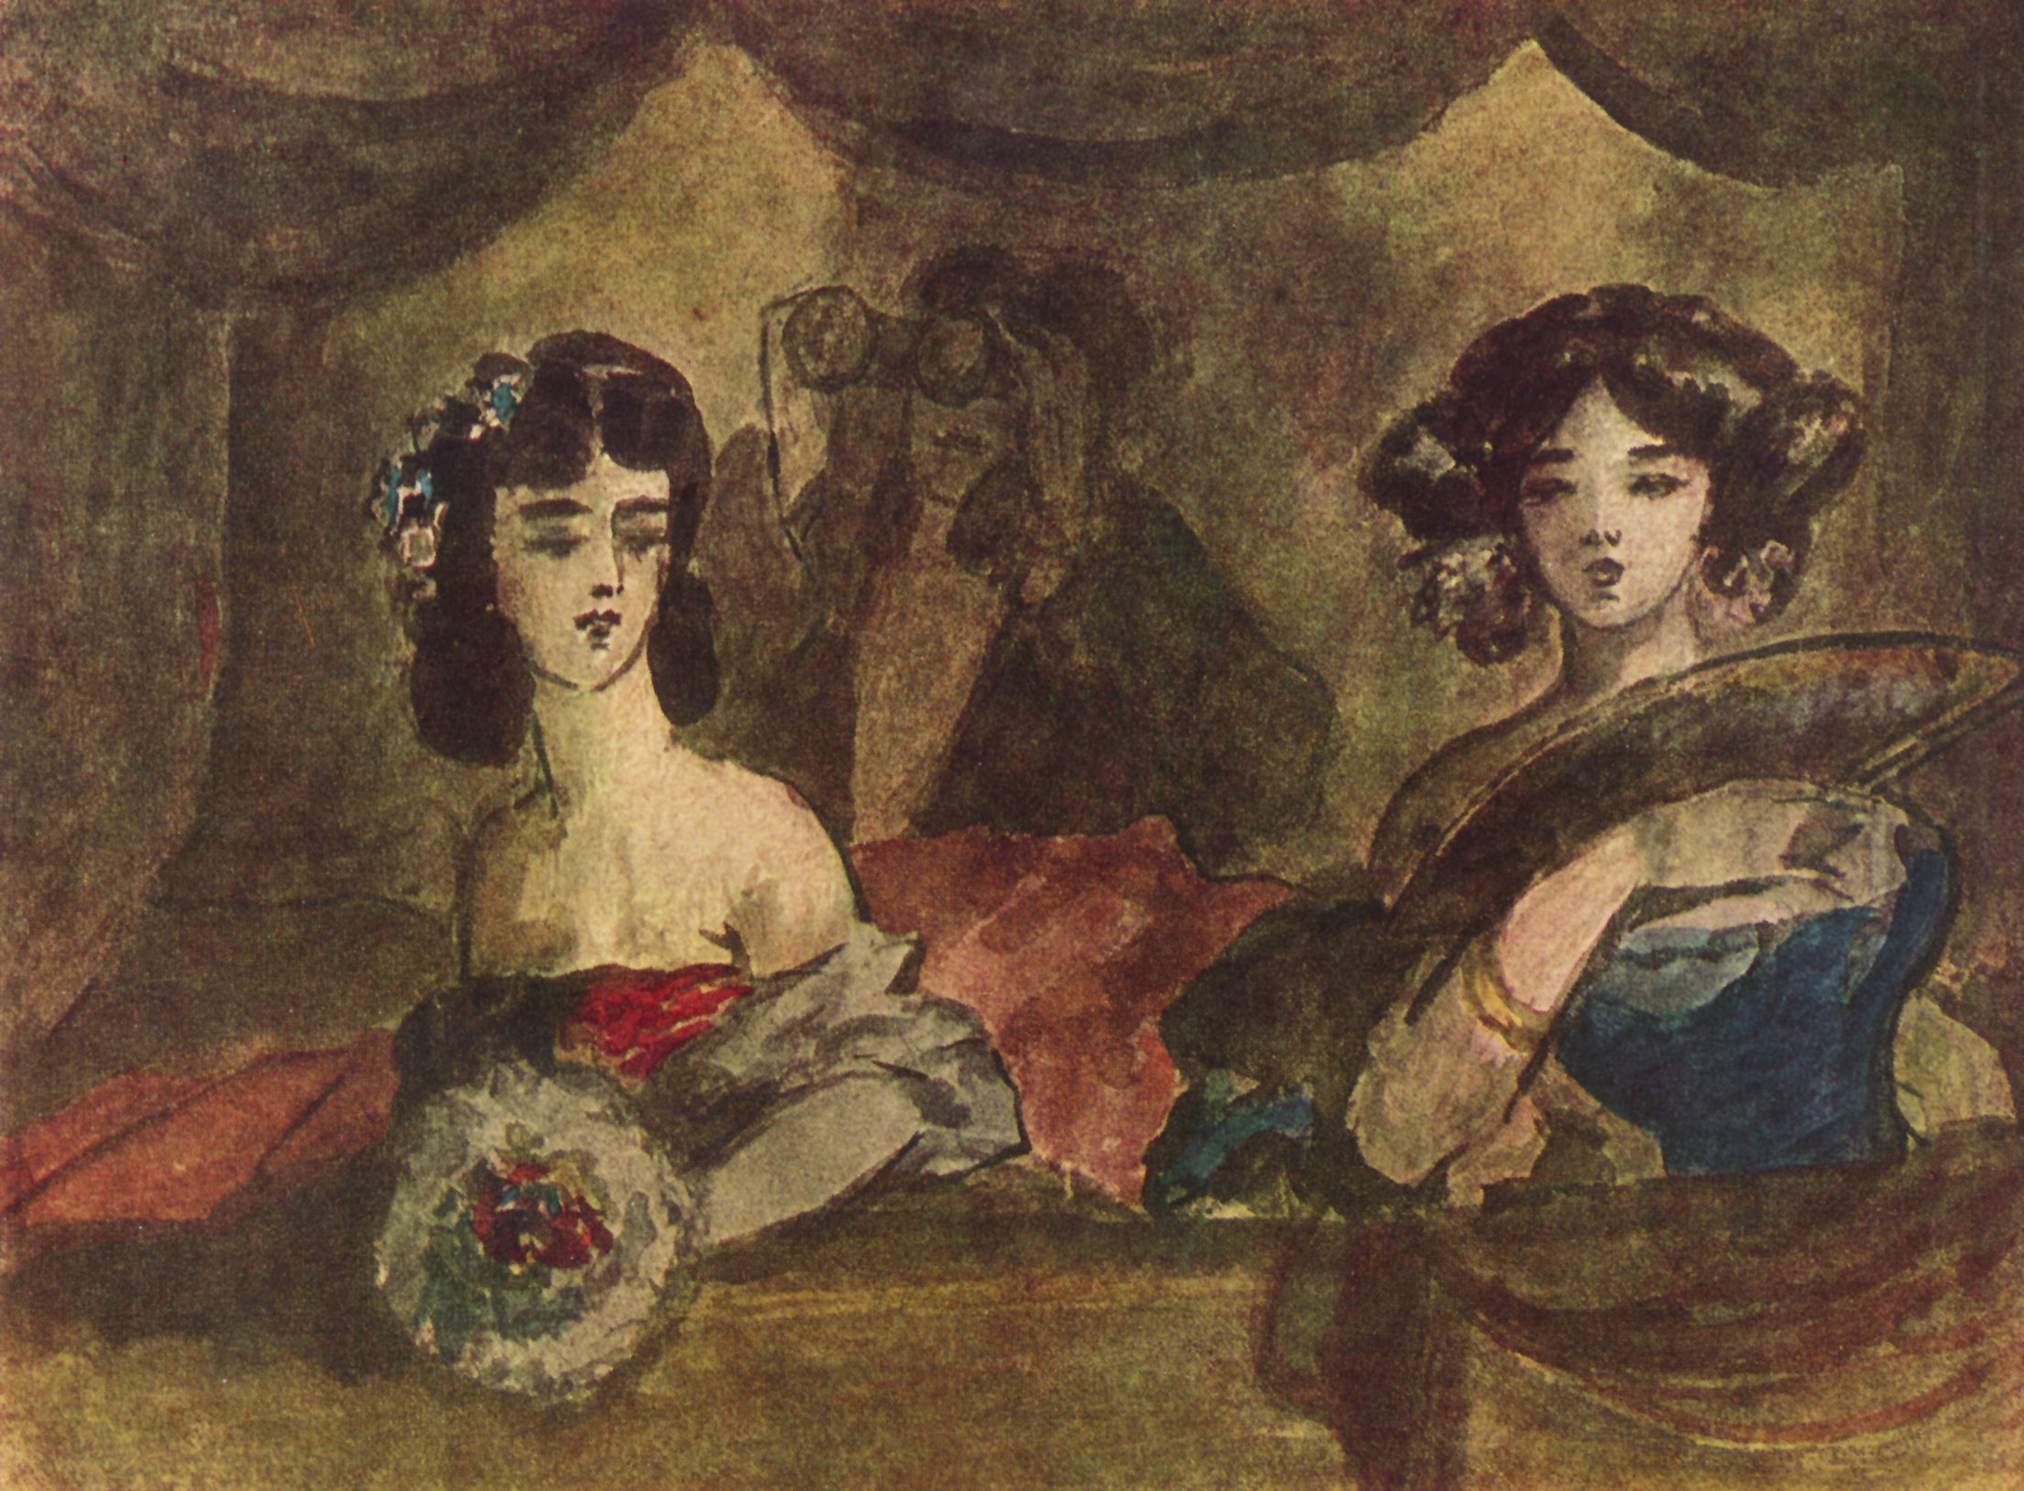
\includegraphics{Constantin-Ernest-Adolphe-Hyacinthe_Guys_001.jpg}}
\end{myframe}


\begin{myframe}
\pictitle{Un bar aux Folies Bergère (A Bar at the Folies-Bergère, Бар в «Фоли-Бержер»)}{Édouard Manet, 1882}{Courtauld Gallery, London}{http://en.wikipedia.org/wiki/File:Edouard_Manet,_A_Bar_at_the_Folies-Bergère.jpg}

\resizebox{.88\textwidth}{!}{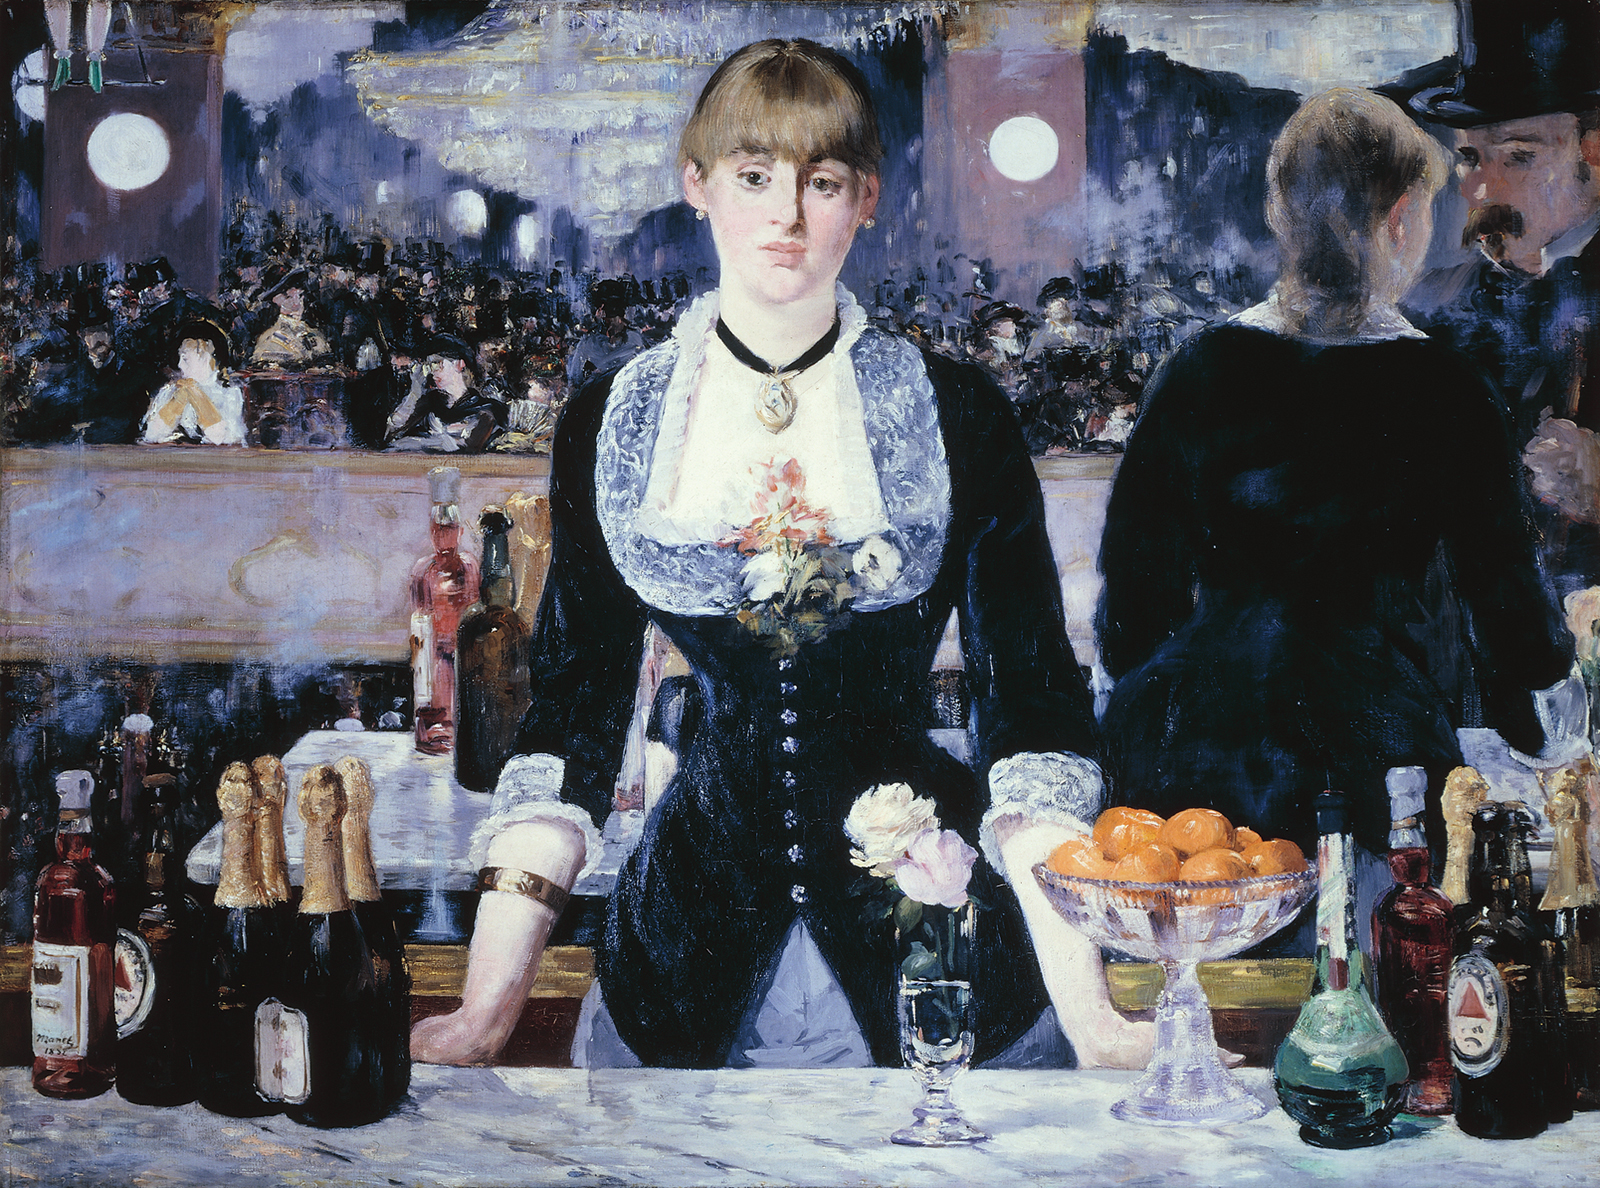
\includegraphics{Edouard_Manet,_A_Bar_at_the_Folies-Bergere.jpg}}
\end{myframe}


\end{document}
